\section{Games}
In mathematical terms a game is a graph, often a tree. The nodes are similar to the configurations of a turing machine, and he edges (the possibile moves of a player) are similar to the transitions of a nondeterministic turing machine. 
Tris Example:
\begin{figure}[h]
    \centering
    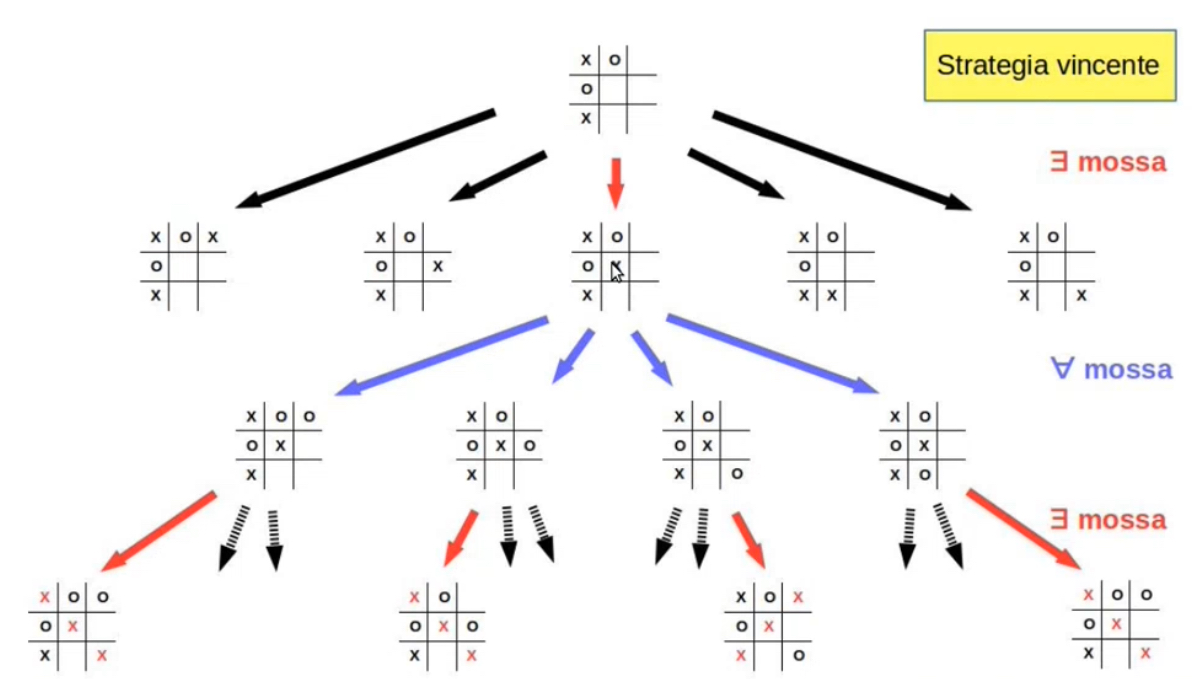
\includegraphics[width=1\textwidth]{img/tris.jpeg}
    \caption{Tris game}
\end{figure}
\\
It is quite clear that there is an analogy between the study of the games strategies and the quantifiers alternation of QBF which characterize the PSPACE complexity classe.
Games with a constant umber of configurations like tris are not very interesting, but e.g the game of chess which has a fixed number of configurations is very interesting because the number of configurations is comparable to the number of atoms in the universe. We still don't know if there is a winning strategy for the first player or not. In the complexity theory we are more interested in games with a variable number of configurations. An in interesting aspect is: what is a solution?It must represent in a compact way the winning strategy of a player. That is, what to do in a exponential number of possibile situations. Let's consider the game of Geography. In this game the first player must say the name of a city, the second player must say the name of a city that starts with the last letter of the first city. The game ends when a player cannot find a city. A possibile generalization of this game could be a graph $G=(V,E)$ where the nodes are the cities and the edges are the connections between them. If $(x,y)\in E$ then the player can say $y$ if the previous player said $x$.
\begin{defbox}[Theorem]
    GEOGRAPHY is \textbf{PSPACE}-complete.
\end{defbox} 
Another interesting game is GO. In this game there is a board of $191times 19$, and the two players alternately place black and white pieces on the board. When a pies is surrounded by the pieces of the other player, it is removed from the board. The game ends when no player can place any more pieces on the board. The winner is the player with the most pieces on the board. 
\begin{figure}[h]
    \centering
    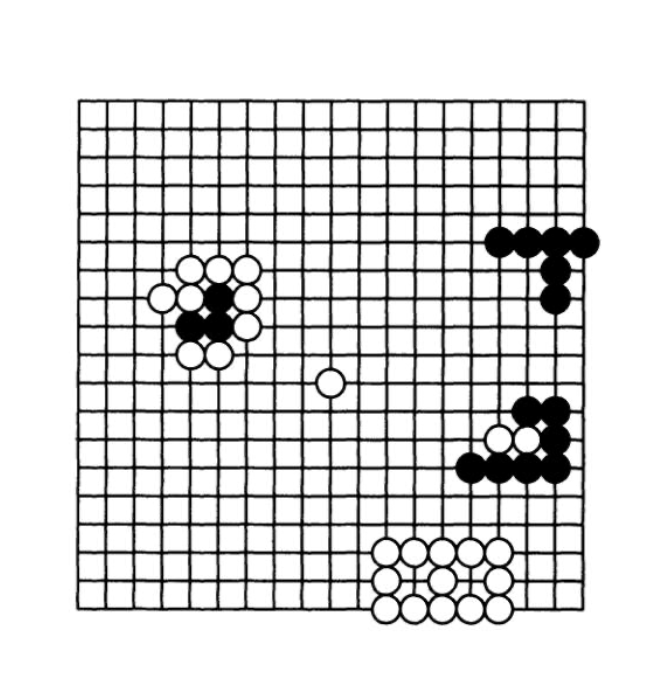
\includegraphics[width=1\textwidth]{img/go.png}
    \caption{GO game}
\end{figure}
\\
To generalize this game we can consider a board of $n\times n$ and decide whether the first player has a winning strategy.
\begin{defbox}[Theorem]
    GO is \textbf{PSPACE}-complete.
\end{defbox}
\subsection{Exercises}
\textbf{Geography can be reduced to the problem of finding a truth assignment in a QBF $\phi$?} Yes, because there is a reduction from Geography to QSAT. That is, given any instance of Geography, we can construct $\phi$ such that is satisfiable if and only if the first player has a winning strategy. I also know that $\phi$ can be constructed in logarithmic space since there is a reduction.
\textbf{If yes, tell if there exists a unique $k$ that upper-bounds the alternation of quantifiers in $\phi$ for every instance of Geography.} We don't know and if it were the case then the polynomial hierarchy and PSPACE would collapse to $\Sigma_k\mathbf{P}$.

